\subsection{Mô hình hóa convolution cho không gian tổng quát}
\subsubsection{Tích chập trên miền số thực}

Đầu tiên, báo cáo sẽ mô hình hóa convolution với một ví dụ đơn giải nhất là trên trường số thực. Giả sử ta tính tích chập hai hàm $x$ và $\psi$ kí hiệu là $(x \star \psi)(u)$, khi đó bản chất ta tính tích chập giữa hai hàm này là ta shift hàm $\psi$ trên trục số thực rồi nhân với hàm $x$\cite{geometricdeep2022}, ta kí hiệu phép shift này là $T_u\psi$. Do đó, ta có công thức của phép tính tích chập trên miền số thực như sau:

\begin{center}
    \scalebox{1.5}{($x \star \psi)(u) =  \langle x, T_u \psi \rangle = \int_{-\infty}^{+\infty} x(v)\psi(u-v) dv $}
\end{center}

Để tổng quát hơn, báo cáo sẽ đưa phép shift này thành tác động của nhóm các phép dịch chuyển gọi là $G$, do đó, miền lấy tích phân sẽ là miền giá trị đầu vào của hai hàm $x$ và $\psi$ gọi là $\Omega$. Cuối cùng, ta có công thức sau:

\begin{center}
    \scalebox{1.5}{$(x \star \psi)(g) =  \langle x, \rho(g) \psi \rangle = \int_{\Omega} x(v)\psi(g^{-1}v) dv$}
\end{center}

Tuy nhiên, đây mới chỉ là phép tích chập cho miền số thực, cho nên, tiếp theo báo cáo sẽ trình bày phép tích chập cho các miền không không gian tổng quát hơn.

\subsubsection{Tích chập trên mặt cầu}
Mạng nơ-ron tích chập (CNN) đã trở thành phương pháp được lựa chọn cho các bài toán học liên quan đến ảnh phẳng 2D. Tuy nhiên, một số vấn đề của sự quan tâm gần đây đã tạo ra nhu cầu về các mô hình có thể phân tích hình ảnh hình cầu\cite{cohen2018sphericalcnns}. Ví dụ bao gồm tầm nhìn đa hướng cho máy bay không người lái, robot và ô tô tự hành, bài toán hồi quy phân tử, và mô hình thời tiết và khí hậu toàn cầu. Một ứng dụng đơn giản của mạng tích chập vào phép chiếu phẳng của tín hiệu hình cầu chắc chắn sẽ thất bại, bởi vì các biến dạng thay đổi theo không gian được tạo ra bởi tín hiệu đó một phép chiếu sẽ làm cho việc chia sẻ trọng số tịnh tiến không hiệu quả\cite{cohen2018sphericalcnns}. Do đó, ta sẽ cần phải định nghĩa được phép tích chập mới trên tín hiệu hình cầu.

\begin{figure}[H]
    \centering
    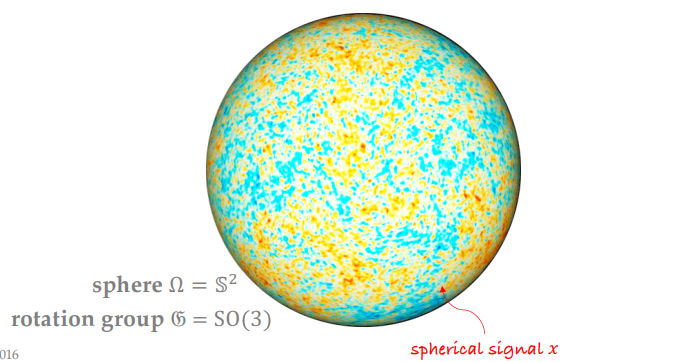
\includegraphics[width=0.7\linewidth]{Images/GDL/sphere_conv/sphere_img.png}
    \caption{Ví dụ minh họa về dữ liệu dạng Sphere\cite{geometricdeep2022}}
\end{figure}

Ta mong muốn có thể định nghĩa tích chập trên miền mặt cầu $S_2$ nhưng khi ta tác động một phép quay lên hình cầu này thì các tín hiệu cầu sẽ bị thay đổi vị trí. Do đó, đầu ra của phép tích chập này sẽ là một hàm theo phép quay $R$:
\begin{center}
    \scalebox{1.5}{$(x\ast \psi )(R)=\int_{S^2}x(u)\psi (R^{-1}u)du$}
\end{center}

Phép quay $R$ ở đây bản chất là ta di chuyển vị trí $u$ đến vị trí $v$ trên mặt cầu $S_2$ và tác động phép quay này chính là tác động của nhóm $SO(3)$. Tuy nhiên, trong $SO(3)$ thì có rất nhiều phép quay để đi từ vị trí $u$ đến vị trí $v$, do đó, ta cần phải tính thêm tích chập trên nhóm $SO(3)$. Khi đó, ta có công thức tính tích chập như sau:

\begin{center}
    \scalebox{1.5}{$((x\ast\psi)\ast\phi)(R)=\int_{SO(3)}(x\ast\psi)(Q)\phi(R^{-1}Q)dQ$}
\end{center}

Để thấy được sự hữu dụng của phép tích chập trên mặt cầu, báo cáo sẽ đưa ra một số ứng dụng củ thể của chúng. Cụ thể hơn, báo cáo sẽ đưa ra một số thực nghiệm của một bài báo nổi tiếng là \textit{Spherical CNN}\cite{cohen2018sphericalcnns}.

Đầu tiên là thực nghiệm so sánh hiệu suất phân loại của \textit{Spherical CNN} với mạng CNN phẳng trên bộ dữ liệu MNIST được chiếu lên mặt cầu. Kết quả cho thấy \textit{Spherical CNN} đạt độ chính xác 96\% trên tập kiểm tra xoay khi được huấn luyện trên tập huấn luyện xoay, trong khi CNN phẳng chỉ đạt 23\%\cite{cohen2018sphericalcnns}. Điều này chứng tỏ khả năng học biểu diễn bất biến xoay vượt trội của \textit{Spherical CNN}.

Tiếp theo, tác giả áp dụng \textit{Spherical CNN} cho bài toán phân loại hình dạng 3D, sử dụng bộ dữ liệu SHREC17 bao gồm các mô hình 3D được xoay ngẫu nhiên. Trên bộ dữ liệu này, \textit{Spherical CNN} đạt điểm F1 là 0.699, chỉ số NDCG là 0.756 và độ chính xác trên tập dữ liệu không xoay là 0.701\cite{cohen2018sphericalcnns}. Kết quả này cho thấy \textit{Spherical CNN} đạt hiệu suất gần như tốt nhất so với các phương pháp hiện đại khác, chứng tỏ tiềm năng của nó trong việc xử lý dữ liệu 3D.

Cuối cùng, tác giả nghiên cứu khả năng của \textit{Spherical CNN} trong việc dự đoán năng lượng nguyên tử hóa của các phân tử dựa trên cấu trúc hình học của chúng. Sử dụng bộ dữ liệu QM7 và biểu diễn các phân tử dưới dạng tín hiệu cầu dựa trên năng lượng Coulomb, \textit{Spherical CNN} đã đạt được RMSE là 8.47 kcal/mol\cite{cohen2018sphericalcnns}. Kết quả này vượt trội hơn hẳn so với các phương pháp dựa trên nhân (RMSE từ 10.82 đến 16.06 kcal/mol) và mạng MLP được huấn luyện trên ma trận Coulomb (RMSE là 12.59 kcal/mol)\cite{cohen2018sphericalcnns}.

\subsubsection{Tích chập cho đa tạp}
Manifold được sử dụng trong nhiều lĩnh vực, đặc biệt là trong học máy và xử lý dữ liệu, vì nó giúp chúng ta hiểu rõ hơn về cấu trúc bên trong của dữ liệu phức tạp. Manifold đặc biệt hữu ích đối với 3D shape (hình dạng 3D) vì nó giúp biểu diễn và xử lý các cấu trúc phức tạp trong không gian 3D một cách hiệu quả hơn. 

Ví dụ, để mô hình một con thỏ theo dạng 3D, ta thường dùng cách khối lập phương chồng lên nhau để mô tả hình dạng và thể tích của chúng (hình ảnh con thỏ bên trái của hình \ref{fig:why-mani}). Tuy nhiên, nếu ta không quan tâm bên trong hình dạng này thì việc biểu diễn bằng các khối lặp phương rất lãng phí không gian lưu trữ và tính toán\cite{geometricdeep2022}. Do đó, đa tạp giúp biểu diễn hình dạng 3D một cách hiệu quả hơn bằng cách tập trung vào các bề mặt của đối tượng, bỏ qua các cấu trúc bên trong không cần thiết.

Do đó, ta có thể sử dụng \textit{manifold} để biểu diễn dữ liệu 3D, nơi chỉ các điểm dữ liệu nằm trên bề mặt của đối tượng 3D được lưu trữ và sử dụng để tạo thành mạng lưới tam giác (mesh). Bởi vậy, \textit{manifold} không "lãng phí" tài nguyên để lưu trữ các cấu trúc bên trong, chỉ tập trung vào bề mặt, từ đó tạo ra một biểu diễn nhẹ và hiệu quả hơn\cite{geometricdeep2022} (hình ảnh con thỏ ở giữa trong hình \ref{fig:why-mani}). Đây cũng là cách được áp dụng trong \textit{computer graphic} liên quan đến vật thể 3D.

Hơn thế nữa, \textit{manifold} được sử dụng như một mô hình tự nhiên cho các hình dạng có thể biến dạng (deformable shapes)\cite{geometricdeep2022}. Ví dụ như hình dạng của con người, với các bộ phận có thể co giãn, di chuyển hoặc thay đổi hình dạng, là một ví dụ điển hình về việc sử dụng manifold (hình ảnh bên phải của hình \ref{fig:why-mani}). Do đó, \textit{manifold} phù hợp với các hình dạng có thể biến dạng, vì nó có thể dễ dàng mô phỏng và điều chỉnh các biến dạng mà không làm mất đi tính toàn vẹn của hình dạng ban đầu\cite{geometricdeep2022}.

\begin{figure}[H]
    \centering
    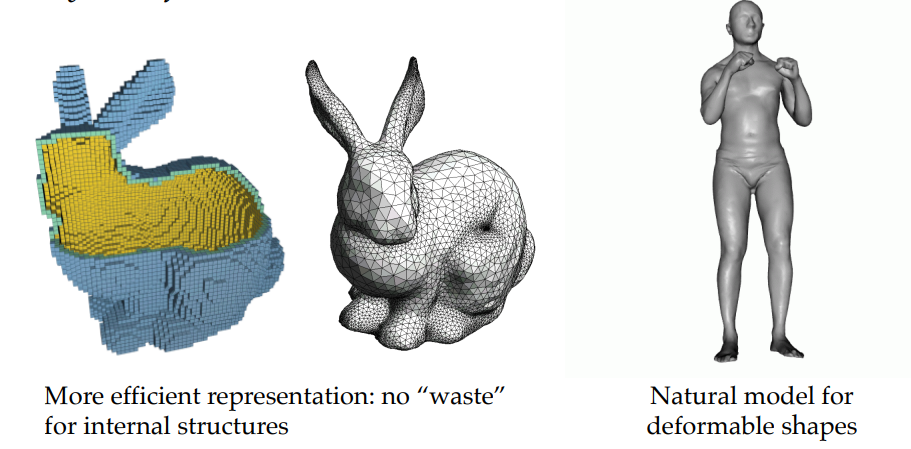
\includegraphics[width=0.8\linewidth]{Images/GDL/manifold_mesh/why_mani.png}
    \caption{Ảnh minh họa dữ liệu đa tạp và meshes\cite{geometricdeep2022}}
    \label{fig:why-mani}
\end{figure}

Tuy nhiên, một ứng dụng quan trọng khác của \textit{manifold} là mô hình hóa protein. Trong quá trình mô hình hóa protein, mục tiêu là biểu diễn các phân tử protein sao cho dễ dàng phân tích các tương tác và biến đổi cấu hình (conformation changes) của chúng. Protein có cấu trúc rất phức tạp với nhiều lớp và các thành phần khác nhau, nhưng không phải tất cả các chi tiết cấu trúc đều quan trọng cho việc nghiên cứu các tương tác chức năng của protein. Dưới đây là hai lý do thể hiện tính hữu ích của \textit{manifold} đối với bài toán này:

\begin{itemize}
    \item Manifold giúp "trừu tượng hóa" (abstract out) các cấu trúc bên trong của protein mà không cần thiết cho việc tương tác. Điều này có nghĩa là chỉ tập trung vào các yếu tố quan trọng như bề mặt của protein, nơi xảy ra các tương tác với các phân tử khác\cite{geometricdeep2022}. Bằng cách này, chúng ta có thể giảm độ phức tạp của mô hình mà không làm mất đi thông tin cần thiết cho việc phân tích.

    \item Protein không phải là những cấu trúc cố định, chúng có thể thay đổi hình dạng hoặc cấu hình để thích ứng với các chức năng sinh học khác nhau. Manifold cung cấp một cách linh hoạt để mô hình hóa những thay đổi này, giữ nguyên tính toàn vẹn của các vùng tương tác quan trọng trong khi cho phép protein thực hiện các biến đổi cấu hình cần thiết\cite{geometricdeep2022}.
\end{itemize}

\begin{figure}[H]
    \centering
    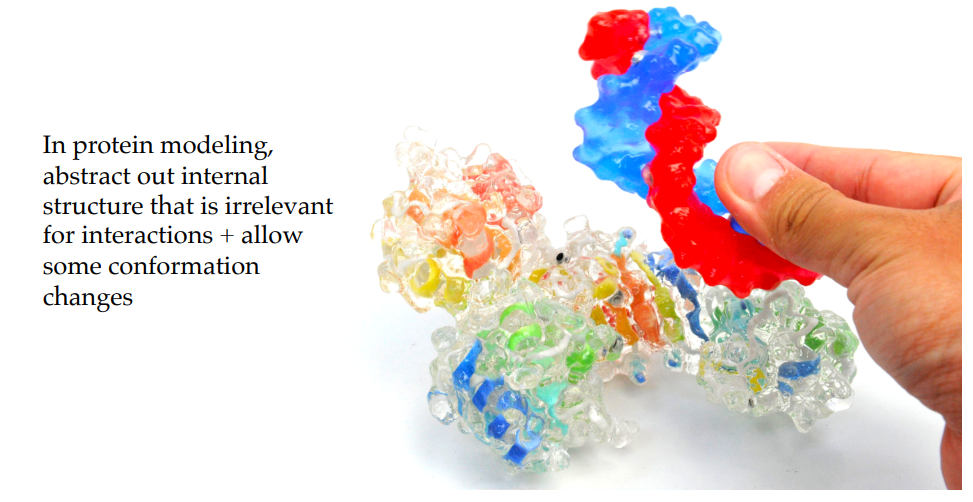
\includegraphics[width=0.85\linewidth]{Images/GDL/manifold_mesh/protein.png}
    \caption{Ảnh minh họa protein\cite{geometricdeep2022}}
    \label{fig:protein}
\end{figure}

Thông thường, nếu ta sử dụng tích chập trên không gian Euclid thì việc ta di chuyển \textit{filter} từ vị trí A đến vị trí B thì đều sẽ cho kết quả như nhau vì chúng đều đến vị trí B và tính tích chập tại đó (hình \ref{fig:ecnn}). Tuy nhiên, đối với \textit{manifold} thì lại lại khác vì nếu ta đi từ A đến B theo hai con đường khác nhau thì \textit{filter} sẽ bị thay đổi hướng ban đầu và do đó kết quả tính tích chập tại vị trí B sẽ khác nhau. Để thể hiện rõ điều này, báo cáo sẽ đưa ra hai ví dụ sau:
\begin{itemize}
    \item Tích chập trên hình cầu: Hình \ref{fig:sp_cnn_ex} cho thấy hướng của \textit{filter} khác nhau của hai đường đi khác nhau mặc dù chúng có cùng điểm xuất phát và điểm đến.

    \item Tích chập trên mặt \textit{mobius}: Hình \ref{fig:mobius_ex} cho thấy \textit{filter} của đường đi thứ 2 đã bị lật ngược lại so với đường đi đầu tiên mặc dù chúng có cùng điểm xuất phát và điểm đến.
\end{itemize}

\begin{figure}[H]
    \centering
    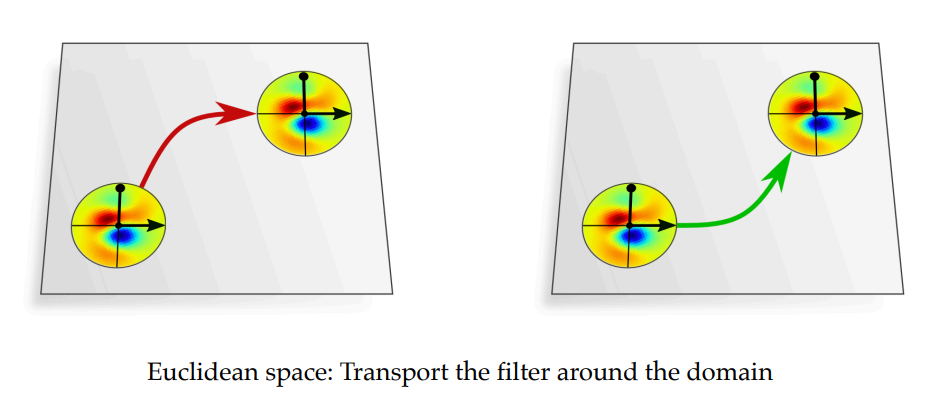
\includegraphics[width=1\linewidth]{Images/GDL/manifold_mesh/E_CNN.png}
    \caption{Ảnh minh họa tích đường đi của \textit{filter} trên không gian Euclid\cite{geometricdeep2022}}
    \label{fig:ecnn}
\end{figure}

\begin{figure}[H]
    \centering
    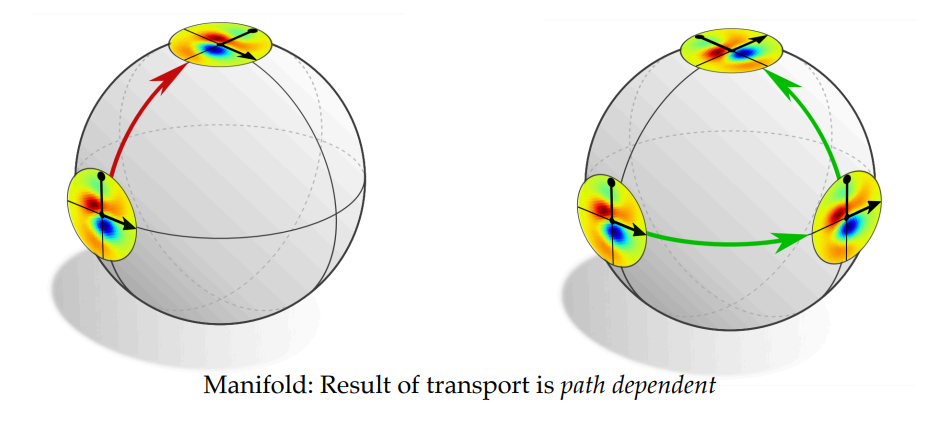
\includegraphics[width=1\linewidth]{Images/GDL/manifold_mesh/sp_cnn_ex.png}
    \caption{Ảnh minh họa tích đường đi của \textit{filter} trên \textit{sphere}\cite{geometricdeep2022}}
    \label{fig:sp_cnn_ex}
\end{figure}

\begin{figure}[H]
    \centering
    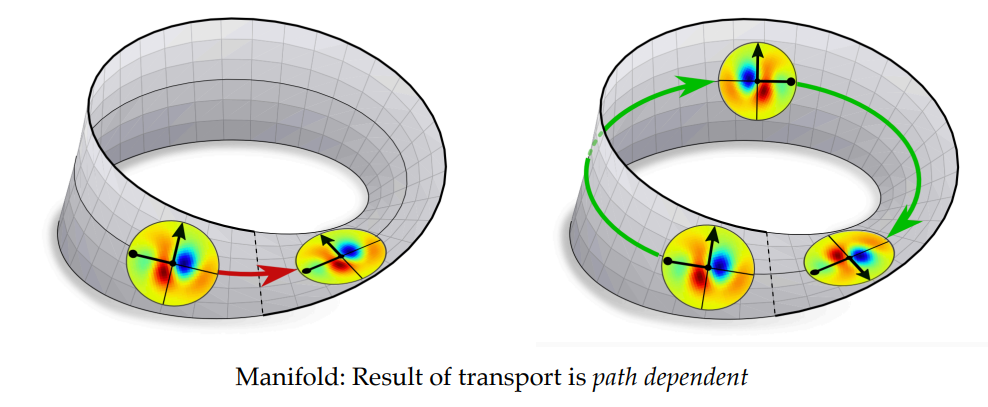
\includegraphics[width=1\linewidth]{Images/GDL/manifold_mesh/mobius_ex.png}
    \caption{Ảnh minh họa tích đường đi của \textit{filter} trên mặt \textit{mobius}\cite{geometricdeep2022}}
    \label{fig:mobius_ex}
\end{figure}

Đối với dữ liệu \textit{manifold}, có hai dạng \textit{invariant} dưới các tác động nhóm như sau:
\begin{itemize}
    \item Biến đổi cục bộ gauge: đây là tác động mà chỉ làm thay đổi tính chất cục bộ của đa tạp mà không ảnh hưởng đến hình dạng tổng thể\cite{geometricdeep2022}. Ví dụ, ta có thể co bóp bụng và điều này làm thay đổi cấu trúc vùng bụng của chúng ta tuy nhiên về mặt tổng thể thì điều này không làm ảnh hưởng đến chúng ta là ai (hình bên trái của hình \ref{fig:local_global_inv}).

    \item Biến đổi toàn cục: đây là tác động làm thay đổi toàn bộ hình dạng của đối tượng, như việc cơ thể người có thể bị kéo giãn, co lại hoặc thay đổi tư thế, tuy nhiên điều này không làm thay đổi đối tượng đấy là gì \cite{geometricdeep2022}. Ví dụ như người A béo lên thì đây chính là tác động làm toàn bộ cơ thể bị thay đổi nhưng về bản chất thì người A vẫn là người A mà không bị biến đổi thành người khác (hai hình bên phải hình \ref{fig:local_global_inv}).
\end{itemize}

\begin{figure}[H]
    \centering
    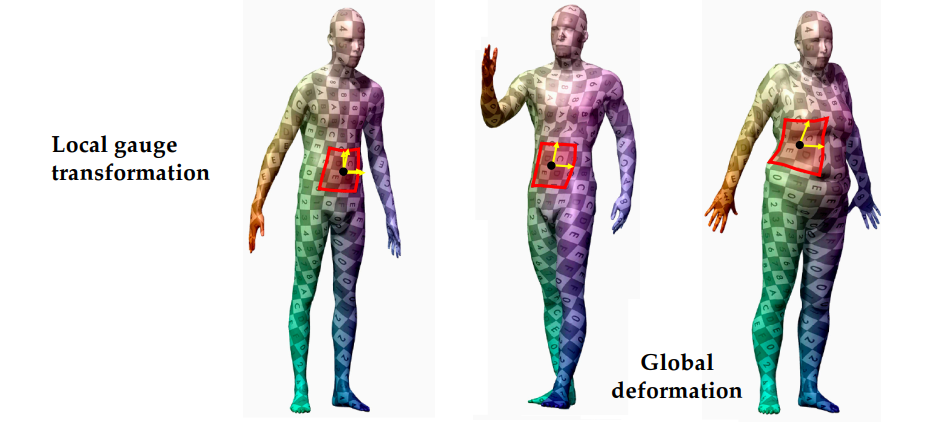
\includegraphics[width=1\linewidth]{Images/GDL/manifold_mesh/local_global_inv.png}
    \caption{Ảnh minh họa hai dạng \textit{invariant} đối với dữ liệu \textit{manifold}\cite{geometricdeep2022}}
    \label{fig:local_global_inv}
\end{figure}

Bây giờ, vấn đề được đặt ra cho việc tính tích chập trên đa tạp là chúng ta cần định nghĩa \textit{filter}. Rất may là đối với đa tạp thì locally ta có thể biểu diễn chúng lên không gian tiếp xúc tại một điểm trên đa tạp (\textit{tangent space}) và nó đẳng cấu với không gian $R^2$. Do đó, ta có thể định nghĩa được filter trên không gian này. Khi đó, ta định nghĩa công thức tính tích chập trên \textit{manifold} như sau:

\begin{center}
    \scalebox{1.5}{$(x \ast \psi)(u) = \int_{T_u \Omega} \psi(v) x(\exp_u v) dv$}
\end{center}
trong đó:
\begin{itemize}
    \item $T_u \Omega$ là không gian tiếp xúc (\textit{tangent space}) tại điểm $u$ trên đa tạp

    \item $\exp_u$ là một phép ánh xạ nội tại nhằm ánh xạ một điểm trong \textit{tangent space} sang một đa tạp $\Omega$
\end{itemize}
tuy nhiên, có một điểm cần lưu ý ở đây là filter của chúng ta sẽ phải invariant với các phép biến đổi đẳng metric (\textit{isometries}).

Ở công thức trên báo cáo đã xây dựng được công thức tính tích chập cho \textit{manifold}, tuy nhiên vector $\mathbf{v}$ trong công thức là một vector trừu tượng, nghĩa là vector này chưa có tọa độ, cho nên phép ánh xạ $\exp_u$ không thể ánh xạ $\mathbf{v}$ sang $manifold$. Do đó, ta cần phải cho $\mathbf{v}$ tọa độ trong $\mathbb{R}^2$ và có một phép biến đổi để ánh xạ $\mathbf{v}$ vào không gian tiếp xúc $T_u \Omega$ - ta gọi phép ánh xạ này là $\omega_u$. Khi đó, ta có công thức tính tích chập sau:
\begin{center}
    \vspace{-0.5cm}
    \scalebox{1.5}{$(x \ast \psi)(u) = \int_{\mathbb{R}^2} \psi(\mathbf{v}) x(\exp_u \omega_u \mathbf{v}) d\mathbf{v}$}
\end{center}
\vspace{-0.5cm}
Tuy nhiên, đây chỉ là công thức cho việc tính tích chập khi chưa có tác động của một nhóm. Do đó, ta sẽ cần xây dựng công thức cho phép biến đổi này, cụ thể hơn là phép biến đổi cục bộ (\textit{gauge transform}). Ta ký hiệu phép biến đổi này như sau:
\begin{center}
    \vspace{-0.5cm}
    \scalebox{1.5}{$g: \Omega \rightarrow SO(2)$}
\end{center}
\vspace{-0.5cm}
Cuối cùng, ta có công thức tính tích chập dưới tác động của một nhóm như sau:
\begin{center}
    \scalebox{1.5}{$(x \star \psi)(u) = \int_{\mathbb{R}^2} \psi(v) \rho(g) x(\exp_u\omega_u v) d{\bf{v}}$}
\end{center}
trong đó, \textit{filter} sẽ phải \textit{equivariant} đối với \textit{gauge transform}, nghĩa là:
\begin{center}
    \scalebox{1.5}{$\psi(g^{-1} {\bf{v}}) = \rho(g^{-1}) \psi({\bf{v}}) \rho(g)$}
\end{center}
\begin{figure}[H]
    \centering
    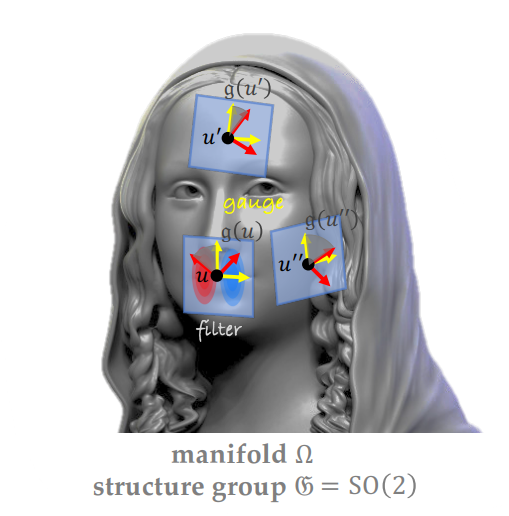
\includegraphics[width=0.7\linewidth]{Images/GDL/manifold_mesh/mani_cnn/mani_cnn.png}
    \caption{Ảnh minh họa filter trên đa tạp có tác động của một nhóm\cite{geometricdeep2022}}
\end{figure}

Tiếp theo, báo cáo sẽ đưa ra một số ứng dụng thực tế của tích chập trên đa tạp. Một ứng dụng gần gũi với chúng ta nhất đấy là làm đồ họa 3D cho game. Ở đây, việc chúng ta cần làm là chuyển đổi các chuyển động mẫu của khuôn mặt người vào trong đồ họa máy tính.

\begin{figure}[H]
    \centering
    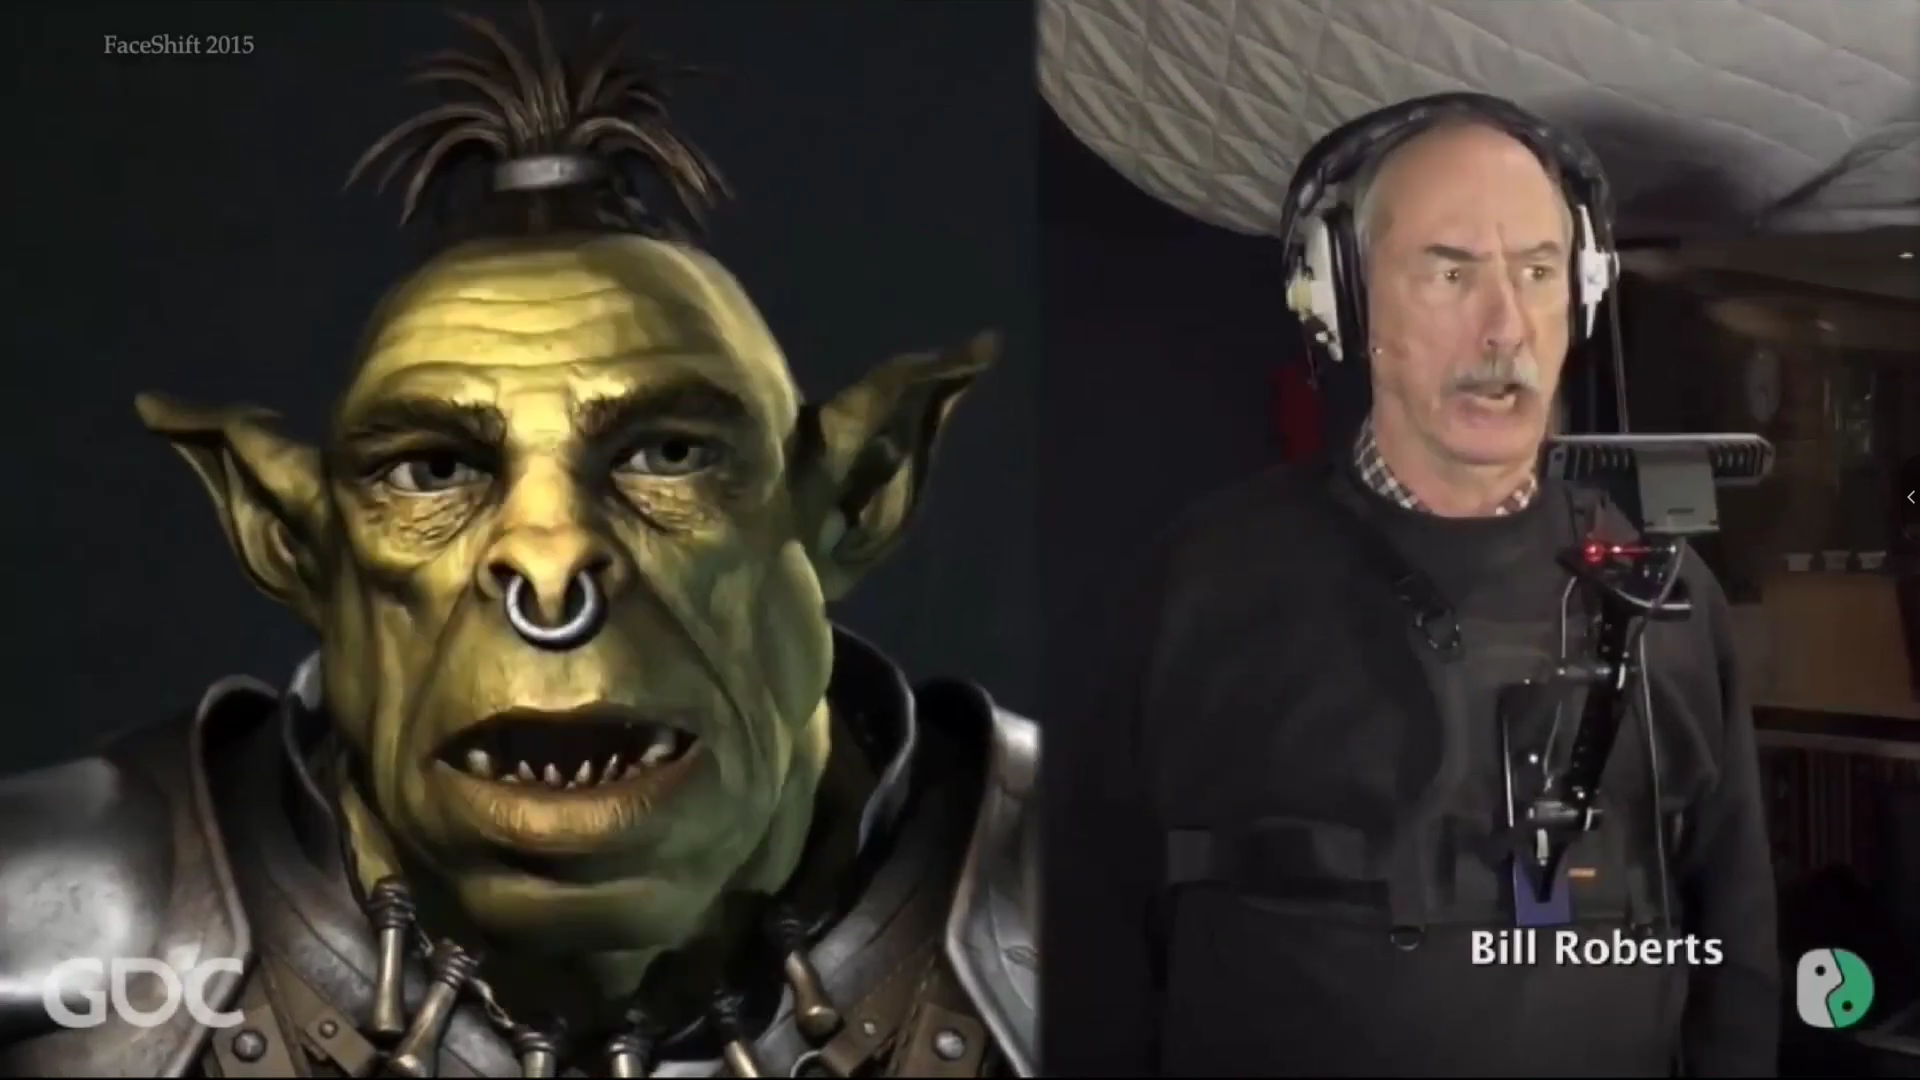
\includegraphics[width=0.7\linewidth]{Images/GDL/manifold_mesh/mani_cnn/app_mani.png}
    \caption{Ứng dụng của tích chập cho manifold trong computer graphic\cite{geometricdeep2022}}
\end{figure}

Để có thể chuyển được các chuyển động của khuôn mặt sang cho nhân vật trong đồ họa máy tính, đầu tiên là ta sẽ cần phải scan khuôn mặt người thật liên tục để có được input 3D. Khi đó, ta cần ánh xạ đầu vào này vào một khuôn mặt dạng mesh tiêu chuẩn rồi bắt đầu thực hiện các phép biến đổi trên đó để hình thành được chuyển động của khuôn mặt. Tuy nhiên, đầu vào 3D sau khi scan có khá là nhiều nhiễu và do đó, ta cần phải sử dụng mesh-convolution để có thể ánh xạ chính xác nhất có thể từ đầu vào sang khuôn mặt dạng mesh tiêu chuẩn\cite{geometricdeep2022}.

\begin{figure}[H]
    \centering
    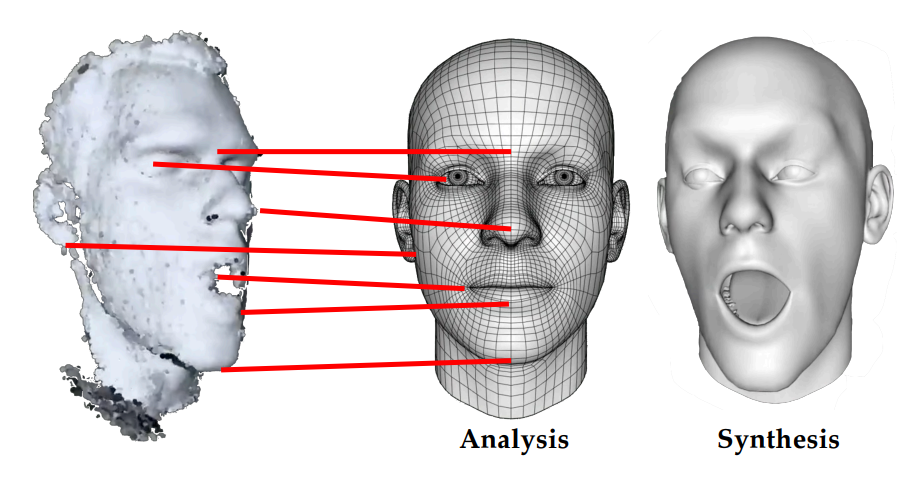
\includegraphics[width=0.7\linewidth]{Images/GDL/manifold_mesh/mani_cnn/computer_graphic.png}
    \caption{Tổng quan quá trình đưa chuyển động của khuôn mặt vào trong đồ họa máy tính\cite{geometricdeep2022}}
\end{figure}

Một ứng dụng khác của tích chập trên đa tạp đó là tái cấu trúc lại hình dạng 3D từ một hình ảnh 2D. Nghĩa là đầu vào sẽ là một hình ảnh và đầu ra sẽ là hình dạng 3D của vật thể trong hình ảnh đấy\cite{geometricdeep2022}.

\begin{figure}[H]
    \centering
    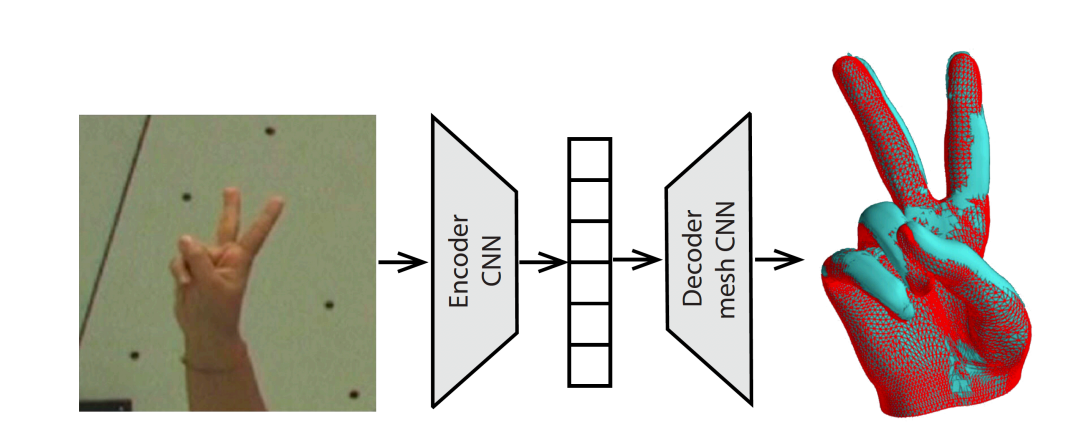
\includegraphics[width=1\linewidth]{Images/GDL/manifold_mesh/mani_cnn/3d_hand.png}
    \caption{Ứng dụng tái cấu trúc lại hình dạng 3D của một vật thể từ một hình ảnh\cite{geometricdeep2022}}
\end{figure}
